\documentclass[xcolor={rgb,x11names,svgnames},rgb,x11names,svgnames]{beamer}

%\includeonlyframes{alg}

\usepackage[T1]{fontenc}
\usepackage{cellspace}

\usepackage{amsmath}
\usepackage{amsfonts}
\usepackage{tikz}
\usepackage{xspace}
\usepackage[normalem]{ulem}
\usepackage{minted}
\definecolor{codebg}{rgb}{0.95,0.95,0.95}
\setminted{bgcolor=codebg}
\usepackage{changepage}

\newenvironment{wider}{%
\begin{adjustwidth}{-0.6cm}{}%
  \begin{minipage}{12cm}%
}{%
\end{minipage}%
\end{adjustwidth}%
}

\usepackage{ifthen}


\usepackage{marvosym}
\usepackage{pifont}
%\usepackage[rgb]{xcolor}

\newcommand{\bigO}[1]{\ensuremath{\mathcal{O}\left( #1 \right)} }
\newcommand{\bigOmega}[1]{\ensuremath{\Omega\left( #1 \right)} }

\newcommand{\red}{\alert}
\newcommand{\green}{\color{LimeGreen}}
\newcommand{\blue}{\color{cyan}}

% FORTIN
\newcommand{\mynote}[1]{\note<1>[item]{#1}}
\newcommand{\euro}{\EUR\xspace}

\usetikzlibrary{patterns}
\usetikzlibrary{snakes}
 \usetikzlibrary{arrows}
\usetikzlibrary{backgrounds}
\usetikzlibrary{shapes}
\usetikzlibrary{shadows}
\usetikzlibrary{shadings}
\usetikzlibrary{calc}
\usetikzlibrary{decorations}
\usetikzlibrary{decorations.pathmorphing}
\usetikzlibrary{decorations.shapes}
\usetikzlibrary{decorations.markings}
\usetikzlibrary{positioning}
\usetikzlibrary{math}

\definecolor{amethyst}{rgb}{0.6, 0.4, 0.8}
\definecolor{cyan}{rgb}{0,0.6796875,1}

\usecolortheme{rose}
\setbeamertemplate{footline}{}
\setbeamertemplate{navigation symbols}{}

\usepackage{fontspec}

\setsansfont{PalatinoSansLTPro}[
   Path = /home/charles/charles_work/fonts/PalatinoSans/, 
   Extension      = .otf,
   UprightFont    = *-Regular,
   BoldFont= *-Bold ,
   ItalicFont = *-Italic,
   BoldItalicFont = *-BoldIta
]

\title{Lecture 4: ``Practical'' MPI}

\begin{document}

\begin{frame}[label=title]
  \titlepage
\end{frame}


\section{Généralités}

%%%%%%%%%%%%%%%%%%%%%%%%%%%%%%%%%%%%%%%%%%%%%%%%%%%%%%%%%%%%%%%%%%%%%%
\begin{frame}
\frametitle{How to Write Efficient Parallel Programs?}

\begin{block}{General principles}

\begin{itemize}
\item \textbf{Data locality}: minimize communications by placing data near the CPUs that need them

\medskip

\item \textbf{load balancing}: minimize periods of inactivity

\medskip

\item \textbf{Overlap communication with computation}: avoid processors sitting
  idle while transferring data
\end{itemize}
\end{block}

\end{frame}


%%%%%%%%%%%%%%%%%%%%%%%%%%%%%%%%%%%%%%%%%%%%%%%%%%%%%%%%%%%%%%%%%%%%%%
\begin{frame}
  \frametitle{Load balancing}

  ``Load balancing'' = who does what? = affecting tasks to CPU
  
  \begin{exampleblock}{Predictable workload}
    \begin{itemize}
    \item[$\Rightarrow$] \textbf{Static} job affectation
      \begin{itemize}
      \item[$=$] Can be determined in advance, fixed over time
      \end{itemize}
      
    \item Typical scenario: 
      \begin{itemize}
      \item All data requiring the same amount of computation time
      \item[$\rightarrow$] Distributed by block, cyclic, \dots
      \end{itemize}
    \end{itemize}
  \end{exampleblock}
  
  \medskip
  
  \begin{alertblock}{Unpredictable workload}
    \begin{itemize}
    \item[$\Rightarrow$] \textbf{Dynamic} load balancing
      \begin{itemize}
      \item Affectation of tasks to processes \emph{during} the computation
      \end{itemize}
    \item \sout{Master-slave} Boss-worker paradigm
    \item ``Work stealing'' paradigm
    \end{itemize}
  \end{alertblock}
\end{frame}


%%%%%%%%%%%%%%%%%%%%%%%%%%%%%%%%%%%%%%%%%%%%%%%%%%%%%%%%%%%%%%%%%%%%%%
\begin{frame}
  \frametitle{\sout{Master-Slave} Boss-Worker  Model}

  \begin{itemize}
  \item The boss knows the data and the work to be done
  \item Available workers ask for work
  \item The boss sends tasks (or orders the workers to stop)
    \begin{alertblock}{Limitations}
      \begin{itemize}
      \item The boss needs a lot of RAM if they have to load all the data
      \item 2 message exchanges per task (A/R) $\longrightarrow$ high granularity
      \item Too many workers $\rightarrow$ the boss becomes a bottleneck
      \end{itemize}
    \end{alertblock}
    
    \begin{exampleblock}{Advantages~:}
      \begin{itemize}
      \item Good load balancing, even with heterogeneous resources (or availability/speed that varies with time)
      \item \emph{Checkpointing} is very easy (checkpoint the boss)
      \end{itemize}
    \end{exampleblock}
  \end{itemize}
\end{frame}


%%%%%%%%%%%%%%%%%%%%%%%%%%%%%%%%%%%%%%%%%%%%%%%%%%%%%%%%%%%%%%%%%%%%%%
\begin{frame}
  \frametitle{Work-Stealing Model}

  \begin{exampleblock}{Principle}
    
    \begin{itemize}
    \item Each processor manages their own work list
      
      \begin{itemize}
      \item \textit{A priori} fair initial distribution
      \end{itemize}
      
    \item If task list is empty :
      \begin{itemize}
      \item Choose a \emph{victim} (randomly?)
      \item ``Steal'' a fraction (50\% ?) of the victim's remaining work
      \end{itemize}
    \end{itemize}
  \end{exampleblock}
  
  \bigskip
  
  \begin{itemize}
  \item [+] Completely symmetrical
    \begin{itemize}
    \item ``\textit{No gods, no masters}'' \CircledA
    \end{itemize}
    
  \item [+] Every process participates in the calculation
    \begin{itemize}
    \item No \sout{parasite} bosses twiddling their thumbs
      
    \end{itemize}
  \item [--] not easy to detect when the computation is terminated
  \item [--] difficult to program
  \item [--] difficult to \emph{checkpoint}
  \end{itemize}
\end{frame}

%%%%%%%%%%%%%%%%%%%%%%%%%%%%%%%%%%%%%%%%%%%%%%%%%%%%%%%%%%%%%%%%%%%%%

%%%%%%%%%%%%%%%%%%%%%%%

\begin{frame}
  \frametitle{Overlapping Communication and Computation}

  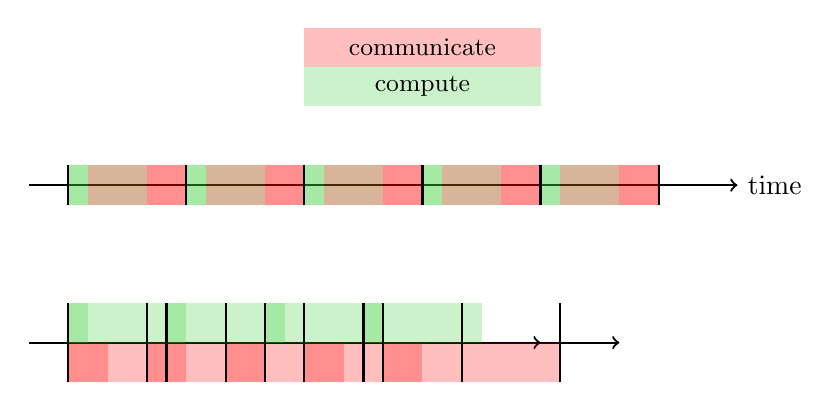
\begin{tikzpicture}
    % initial 
    \draw[thick, ->] (-0.5, 0) -- (8.5, 0) node[right] {time};
    \foreach \i in {0, 1, 2, 3, 4}  {
      % longer comms
      \fill<1>[fill=LimeGreen, nearly transparent] (\i*1.5cm, -0.25) rectangle +(1, 0.5);
      \fill<1>[fill=red, nearly transparent] (\i*1.5cm + 1cm, -0.25) rectangle +(0.5, 0.5);
      % longer comms
      \fill<2>[fill=LimeGreen, nearly transparent] (\i*1.5cm, -0.25) rectangle +(0.25, 0.5);
      \fill<2>[fill=red, nearly transparent] (\i*1.5cm + 0.25cm, -0.25) rectangle +(1.25, 0.5);
    }
    \foreach \i in {0, 1, 2, 3, 4, 5} {
      \draw[thick] (\i*1.5cm, -0.25) -- +(0, 0.5);
    }

    \begin{scope}[yshift=-2cm]
      % overlap, longer compute
      \draw<1>[thick, ->] (-0.5, 0) -- (6, 0);
      \draw<2>[thick, ->] (-0.5, 0) -- (7, 0);
      \foreach \i in {0, 1, 2, 3, 4}  {
        \fill<1>[fill=LimeGreen, nearly transparent] (\i*1cm, 0) rectangle +(1, 0.5);
        \fill<1>[fill=red, nearly transparent] (\i*1cm, -0.5) rectangle +(0.5, 0.5);

        \fill<2>[fill=LimeGreen, nearly transparent] (\i*1.25cm, 0) rectangle +(0.25, 0.5);
        \fill<2>[fill=red, nearly transparent] (\i*1.25cm, -0.5) rectangle +(1.25, 0.5);

      }
      \foreach \i in {0, 1, 2, 3, 4, 5} {
        \draw<1>[thick] (\i*1cm, -0.5) -- +(0, 1);
        \draw<2>[thick] (\i*1.25cm, -0.5) -- +(0, 1);
      }
    \end{scope}
  
    \begin{scope}[xshift=2cm]   % legend
      \fill[fill=LimeGreen, nearly transparent] (1, 1) rectangle +(3, 0.5);
      \path (1, 1) rectangle node[font=\small] {compute} +(3, 0.5);

      \fill[fill=red, nearly transparent] (1, 1.5) rectangle +(3, 0.5);
      \path (1, 1.5) rectangle node[font=\small] {communicate} +(3, 0.5);
    \end{scope}
  \end{tikzpicture}

  \begin{block}{\vspace*{-3ex}}
    \vspace*{-1em}
    \begin{align*}
      T &= T_{comp} + T_{comm} & \text{(before)} \\
      T'&= \max(T_{comp}, T_{comm}) & \text{(after)} \\
        &\geq T/2
    \end{align*}
    \end{block}
\end{frame}

%%%%%%%%%%%%%%%%%%%%%%%%%%%%%%%%%%%%%%%%%%%%%%%%%%%%%%%%%%%%%%%%%%%%%

\begin{frame}[fragile=singleslide]
  \frametitle{Data Parallelism}

  \begin{block}{Classic example: \emph{map}}
\begin{minted}{C}
for (int i = 0; i < n; i++)
         B[i] = f(A[i], i)
\end{minted}
  \end{block}

  \bigskip

  \begin{itemize}
  \item No need for communication / synchronization between processes!
  \item Data distribution?
  \item Load balancing?
  \end{itemize}
\end{frame}

%%%%%%%%%%%%%%%%%%%%%%%%%%%%%%%%%%%%%%%%%%%%%%%%%%%%%%%%%%%%%%%%%

\section{Distribution de données}

\begin{frame}[fragile=singleslide]
\frametitle{1D Distribution}

By blocs:

\medskip

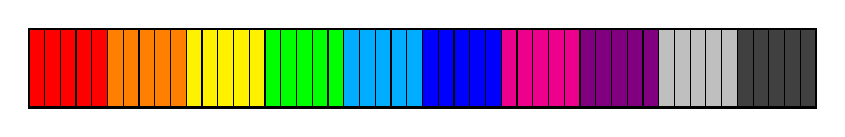
\begin{tikzpicture}
  \filldraw[fill=red]    (0, 0) rectangle  +(1,1);
  \filldraw[fill=orange] (1, 0) rectangle  +(1,1);
  \filldraw[fill=yellow] (2, 0) rectangle  +(1,1);
  \filldraw[fill=green]  (3, 0) rectangle  +(1,1);
  \filldraw[fill=cyan]   (4, 0) rectangle  +(1,1);
  \filldraw[fill=blue]   (5, 0) rectangle  +(1,1);
  \filldraw[fill=magenta] (6, 0) rectangle  +(1,1);
  \filldraw[fill=violet] (7, 0) rectangle +(1,1);
  \filldraw[fill=lightgray] (8, 0) rectangle +(1,1);
  \filldraw[fill=darkgray] (9, 0) rectangle +(1,1);
  
  \draw[thick] (0, 0) rectangle (10, 1);
  \foreach \i in {0.2, 0.4, ..., 9.8}
  \draw (\i, 0) -- +(0, 1);
\end{tikzpicture}

\begin{itemize}
\item Easiest !
\item Favored by MPI
\end{itemize}

\vspace{1cm}

Cyclic

\medskip

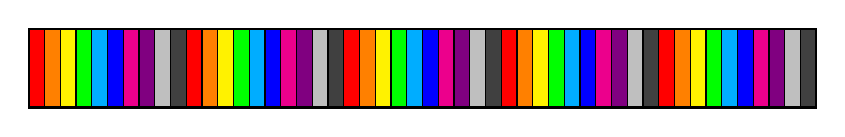
\begin{tikzpicture}
  \foreach \i in {0, 2, 4, 6, 8} {
    \filldraw[fill=red]    (\i, 0) rectangle  +(0.2,1);
    \filldraw[fill=orange]    (\i + 0.2, 0) rectangle  +(0.2,1);
    \filldraw[fill=yellow]    (\i + 0.4, 0) rectangle  +(0.2,1);
    \filldraw[fill=green]    (\i + 0.6, 0) rectangle  +(0.2,1);
    \filldraw[fill=cyan]    (\i + 0.8, 0) rectangle  +(0.2,1);
    \filldraw[fill=blue]    (\i + 1, 0) rectangle  +(0.2,1);
    \filldraw[fill=magenta]    (\i + 1.2, 0) rectangle  +(0.2,1);
    \filldraw[fill=violet]    (\i + 1.4, 0) rectangle  +(0.2,1);
    \filldraw[fill=lightgray]    (\i + 1.6, 0) rectangle  +(0.2,1);
    \filldraw[fill=darkgray]    (\i + 1.8, 0) rectangle  +(0.2,1);
  }
  % \filldraw[fill=red]    (0, 0) rectangle  +(1,1);
  % \filldraw[fill=orange] (1, 0) rectangle  +(1,1);
  % \filldraw[fill=yellow] (2, 0) rectangle  +(1,1);
  % \filldraw[fill=green]  (3, 0) rectangle  +(1,1);
  % \filldraw[fill=cyan]   (4, 0) rectangle  +(1,1);
  % \filldraw[fill=blue]   (5, 0) rectangle  +(1,1);
  % \filldraw[fill=magenta] (6, 0) rectangle  +(1,1);
  % \filldraw[fill=violet] (7, 0) rectangle +(1,1);
  % \filldraw[fill=lightgray] (8, 0) rectangle +(1,1);
  % \filldraw[fill=darkgray] (9, 0) rectangle +(1,1);
  
  \draw[thick] (0, 0) rectangle (10, 1);
  \foreach \i in {0.2, 0.4, ..., 9.8}
  \draw (\i, 0) -- +(0, 1);
\end{tikzpicture}

\begin{itemize}
\item May improve load balancing
\item Also possible with MPI
  \begin{itemize}
  \item Must create ``types'' $\leadsto$ \mintinline{C}{MPI_Type_vector}...
  \end{itemize}
\end{itemize}
\end{frame}

%%%%%%%%%%%%%%%%%%%%%%%%%%%%%%%%%%%%%%%%%%%%%%%%%%%%

\begin{frame}
\frametitle{1D Distribution of 2D Data}

By blocs:

\medskip

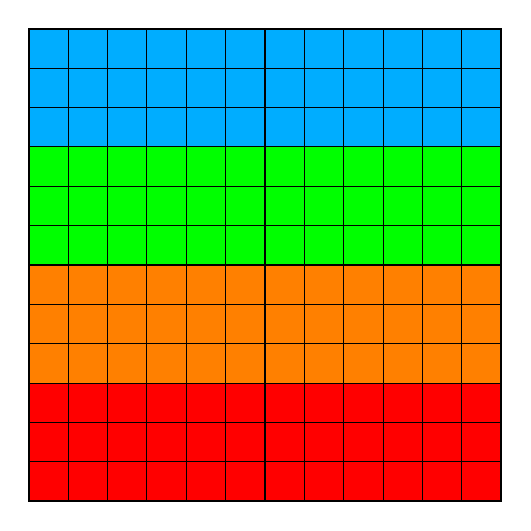
\begin{tikzpicture}[scale=0.5]
  \filldraw[fill=red]    (0, 0) rectangle  +(12,3);
  \filldraw[fill=orange] (0, 3) rectangle  +(12,3);
  \filldraw[fill=green] (0, 6) rectangle  +(12,3);
  \filldraw[fill=cyan]  (0, 9) rectangle  +(12,3);
  
  \draw[thick] (0, 0) rectangle (12, 12);
  \foreach \i in {1, 2, ..., 11} {
    \draw (\i, 0) -- +(0, 12);
    \draw (0, \i) -- +(12, 0);
  }
\end{tikzpicture}
\end{frame}


%%%%%%%%%%%%%%%%%%%%%%%%%%%%%%%%%%%%%%%%%%%%%%%%%%%%

\begin{frame}
\frametitle{1D Distribution of 2D Data}

Cyclic:

\medskip

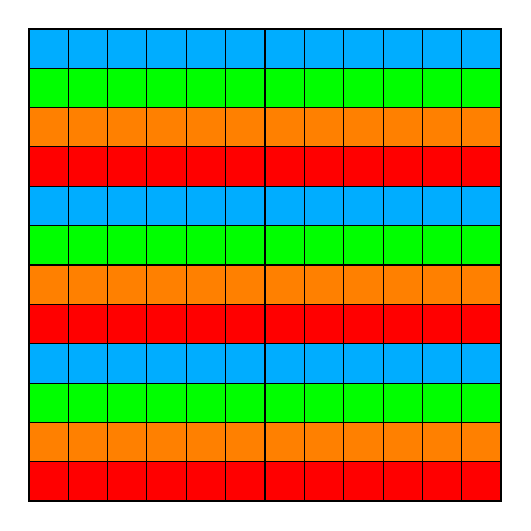
\begin{tikzpicture}[scale=0.5]
  \foreach \i in {0, 4, 8} {
    \filldraw[fill=red]    (0, \i) rectangle  +(12,1);
    \filldraw[fill=orange] (0, 1+\i) rectangle  +(12,1);
    \filldraw[fill=green] (0, 2+\i) rectangle  +(12,1);
    \filldraw[fill=cyan]  (0, 3+\i) rectangle  +(12,1);
  }
  \draw[thick] (0, 0) rectangle (12, 12);
  \foreach \i in {1, 2, ..., 11} {
    \draw (\i, 0) -- +(0, 12);
    \draw (0, \i) -- +(12, 0);
  }
\end{tikzpicture}
\end{frame}

%%%%%%%%%%%%%%%%%%%%%%%%%%%%%%%%

\begin{frame}
\frametitle{2D Distribution of 2D Data}

By blocs:

\medskip

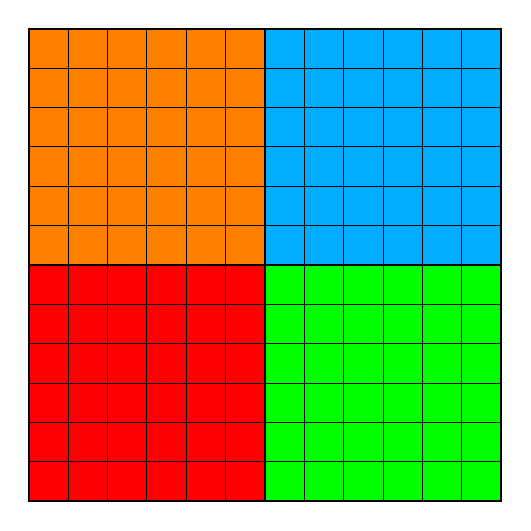
\begin{tikzpicture}[scale=0.5]
  \filldraw[fill=red]    (0, 0) rectangle  +(6, 6);
  \filldraw[fill=orange] (0, 6) rectangle  +(6,6);
  \filldraw[fill=green] (6, 0) rectangle  +(6,6);
  \filldraw[fill=cyan]  (6, 6) rectangle  +(6,6);

  \draw[thick] (0, 0) rectangle (12, 12);
  \foreach \i in {1, 2, ..., 11} {
    \draw (\i, 0) -- +(0, 12);
    \draw (0, \i) -- +(12, 0);
  }
\end{tikzpicture}
\end{frame}

%%%%%%%%%%

\begin{frame}
\frametitle{2D Distribution of 2D Data}

Cyclic:

\medskip

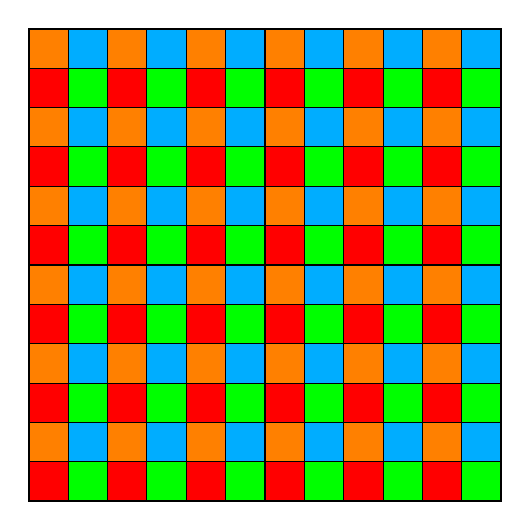
\begin{tikzpicture}[scale=0.5]
  \foreach \i in {0, 2, 4, 6, 8, 10} {
    \foreach \j in {0, 2, 4, 6, 8, 10} {
      \filldraw[fill=red]    (\i, \j) rectangle  +(1, 1);
      \filldraw[fill=orange] (\i, 1+\j) rectangle  +(1,1);
      \filldraw[fill=green] (\i+1, \j) rectangle  +(1,1);
      \filldraw[fill=cyan]  (\i+1, 1+\j) rectangle  +(1,1);
    }
  }
  \draw[thick] (0, 0) rectangle (12, 12);
  \foreach \i in {1, 2, ..., 11} {
    \draw (\i, 0) -- +(0, 12);
    \draw (0, \i) -- +(12, 0);
  }
\end{tikzpicture}
\end{frame}

%%%%%%%%%%%%%%%%%%%%%%%%%%%%%%%%%%%%%%%%%%%%%%%%%%%%%%%%%%%%%%

\begin{frame}
\frametitle{2D Distribution of 2D Data}

Block-Cyclic:

\medskip

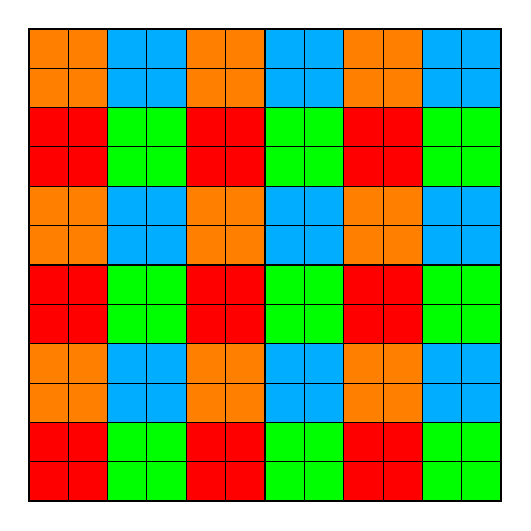
\begin{tikzpicture}[scale=0.5]
  \foreach \i in {0, 4, 8} {
    \foreach \j in {0, 4, 8} {
      \filldraw[fill=red]    (\i, \j) rectangle  +(2, 2);
      \filldraw[fill=orange] (\i, 2+\j) rectangle  +(2,2);
      \filldraw[fill=green] (\i+2, \j) rectangle  +(2,2);
      \filldraw[fill=cyan]  (\i+2, 2+\j) rectangle  +(2,2);
    }
  }
  \draw[thick] (0, 0) rectangle (12, 12);
  \foreach \i in {1, 2, ..., 11} {
    \draw (\i, 0) -- +(0, 12);
    \draw (0, \i) -- +(12, 0);
  }
\end{tikzpicture}
\end{frame}


%%%%%%%%%%%%%%%%%%%%%%%%%%%%%%%%%%%%%%%%%%%%%%%%%%%%%%%%%%%%%%

\begin{frame}
\frametitle{1D Distribution of 3D Data}

\centering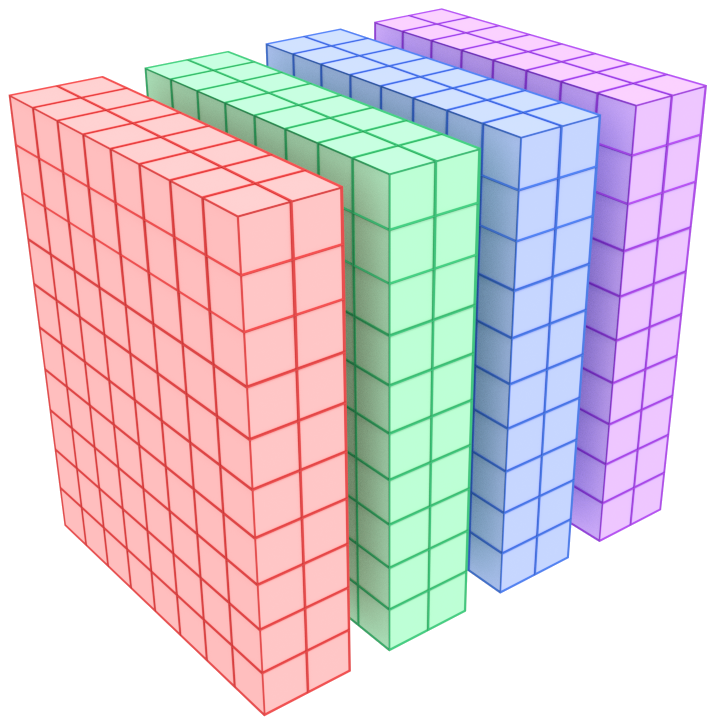
\includegraphics[height=8cm]{slabs.png}

\end{frame}

%%%%%%%%%%%%%%%%%%%%%%%%

\begin{frame}
\frametitle{2D Distribution of 3D Data}

\centering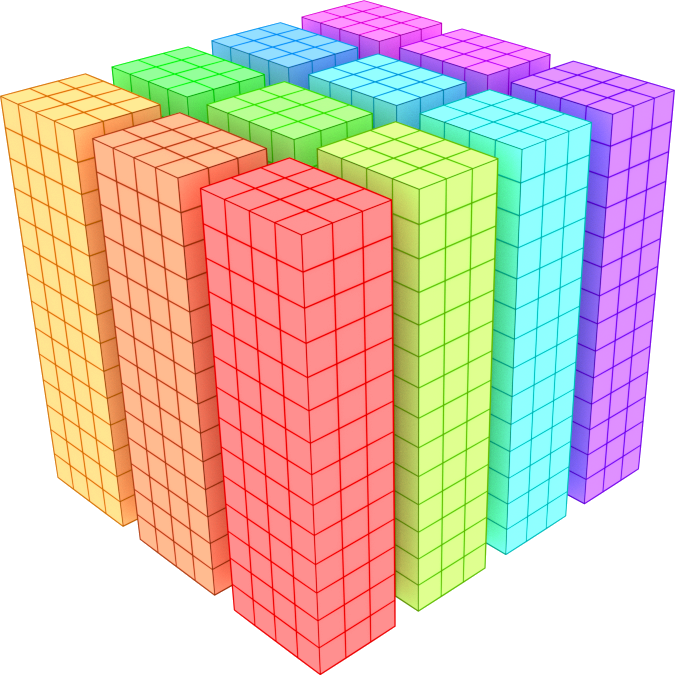
\includegraphics[height=8cm]{pencils.png}

\end{frame}

%%%%%%%%%%%%%%%%%%%%%%%%%

\begin{frame}[fragile=singleslide]
\frametitle{Data Parallelism (continued)}


\begin{block}{Classic example: \emph{reduce}}
\begin{minted}{C}
sum = 0
for (int i = 0; i < n; i++)
    sum = sum + A[i]
\end{minted}
\end{block}

\bigskip

\begin{itemize}
\item Data dependency on \mintinline{C}{sum}? Easy to bypass
\item Distributed memory $\rightarrow$ communications
\item Binomial tree algorithm
\end{itemize}
\end{frame}

%%%%%%%%%%%%%%%%%%%%%%%%%%%%%%%%%%%%%%%%%%%%%%%%%%%%%%%%%%%%%%%%

\begin{frame}[fragile=singleslide]
  \frametitle{MPI in action: \texttt{reduce}}

  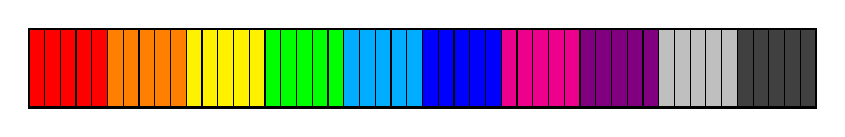
\begin{tikzpicture}
    \filldraw[fill=red]    (0, 0) rectangle  +(1,1);
    \filldraw[fill=orange] (1, 0) rectangle  +(1,1);
    \filldraw[fill=yellow] (2, 0) rectangle  +(1,1);
    \filldraw[fill=green]  (3, 0) rectangle  +(1,1);
    \filldraw[fill=cyan]   (4, 0) rectangle  +(1,1);
    \filldraw[fill=blue]   (5, 0) rectangle  +(1,1);
    \filldraw[fill=magenta] (6, 0) rectangle  +(1,1);
    \filldraw[fill=violet] (7, 0) rectangle +(1,1);
    \filldraw[fill=lightgray] (8, 0) rectangle +(1,1);
    \filldraw[fill=darkgray] (9, 0) rectangle +(1,1);
    \draw[thick] (0, 0) rectangle (10, 1);
    \foreach \i in {0.2, 0.4, ..., 9.8}
    \draw (\i, 0) -- +(0, 1);
  \end{tikzpicture}
  
  \bigskip

\begin{minted}[fontsize=\small]{C}
// Global array of size n
// p processes
int root = 0;
double sum = 0;
for (int i = rank * n / p; (rank + 1) * n / p; i++)
        sum += A[i];
MPI_Reduce(MPI_IN_PLACE, &sum, 1, MPI_DOUBLE, MPI_SUM,
           root, MPI_COMM_WORLD);
\end{minted}        

\begin{align*}
  T &= \frac{n}{p} + \lceil \log_2 p \rceil (\alpha + \beta)
\end{align*}
\end{frame}

%%%%%%%%%%%%%%%%%%%%%%%%%%%%%%%%%%%%%%%%%%%%%%%%%%%%%

% \begin{frame}
% \frametitle{\alert{Shared}-memory \texttt{reduce}}

% \begin{tikzpicture}
%   \filldraw[fill=red]    (0, 0) rectangle  +(1,1);
%   \filldraw[fill=orange] (1, 0) rectangle  +(1,1);
%   \filldraw[fill=yellow] (2, 0) rectangle  +(1,1);
%   \filldraw[fill=green]  (3, 0) rectangle  +(1,1);
%   \filldraw[fill=cyan]   (4, 0) rectangle  +(1,1);
%   \filldraw[fill=blue]   (5, 0) rectangle  +(1,1);
%   \filldraw[fill=magenta] (6, 0) rectangle  +(1,1);
%   \filldraw[fill=violet] (7, 0) rectangle +(1,1);
%   \filldraw[fill=lightgray] (8, 0) rectangle +(1,1);
%   \filldraw[fill=darkgray] (9, 0) rectangle +(1,1);
  
%   \draw[thick] (0, 0) rectangle (10, 1);
%   \foreach \i in {0.2, 0.4, ..., 9.8}
%   \draw (\i, 0) -- +(0, 1);
% \end{tikzpicture}

% \bigskip

% \begin{enumerate}
% \item Tableau \texttt{Scratch} de taille $p$.
% \item $P_i$ fait : $\texttt{Scratch[i]} \gets $ somme de \emph{ses} donnée.
% \item \alert{Barrière}
% \item $P_0$ calcule la somme de \texttt{Scratch} puis l'écrit dans \texttt{sum}
% \item \alert{Barrière}
% \end{enumerate}


% \begin{align*}
%   T &= \frac{n}{p} + p \\
%     &\geq 2 \sqrt{n} & \text{(optimal atteint avec $\sqrt{n}$ processeurs)}
% \end{align*}
% \end{frame}

% %%%%%%%%%%%%%%%%%%%%%%%%%%%%%%%%%%%%%%%%%%%%%%%%%%%%%%%%%%%%%%%%

% \begin{frame}
% \frametitle{Algorithme (mémoire partagée) pour \texttt{reduce}}

% \begin{tikzpicture}
%   \filldraw[fill=red]    (0, 0) rectangle  +(1,1);
%   \filldraw[fill=orange] (1, 0) rectangle  +(1,1);
%   \filldraw[fill=yellow] (2, 0) rectangle  +(1,1);
%   \filldraw[fill=green]  (3, 0) rectangle  +(1,1);
%   \filldraw[fill=cyan]   (4, 0) rectangle  +(1,1);
%   \filldraw[fill=blue]   (5, 0) rectangle  +(1,1);
%   \filldraw[fill=magenta] (6, 0) rectangle  +(1,1);
%   \filldraw[fill=violet] (7, 0) rectangle +(1,1);
%   \filldraw[fill=lightgray] (8, 0) rectangle +(1,1);
%   \filldraw[fill=darkgray] (9, 0) rectangle +(1,1);
  
%   \draw[thick] (0, 0) rectangle (10, 1);
%   \foreach \i in {0.2, 0.4, ..., 9.8}
%   \draw (\i, 0) -- +(0, 1);
% \end{tikzpicture}

% \bigskip

% \begin{block}{$\texttt{reduce}(A, n):$}
%   \begin{enumerate}
%   \item Si $n = 1$, renvoyer $A[0]$.
%   \item Allouer un tableau \texttt{Scratch} de taille $n/2$.
%   \item Pour tout $0 \leq i < n/2$, faire (en parallèle):
%     \begin{itemize}
%     \item $\texttt{Scratch}[i] \gets A[2i] + A[2i+1]$.  
%     \end{itemize}
    
%   \item renvoyer : $\texttt{reduce}(\texttt{Scratch}, n/2)$.
%   \end{enumerate}
% \end{block}

% \begin{align*}
%   T &= \frac{2n}{p} + \log_2 p \\
%     &\geq 1 + \log_2 p & \text{(optimal atteint avec $n/2$ processeurs)}
% \end{align*}
% \end{frame}

\section{EDPs}

%%%%%%%%%%%%%%%%%%%%%%%%%%%%%%%%%%%%%%%%%%%%%%%%%%%%%%%%%%%%%%%%%%%%%

\begin{frame}
\frametitle{Approximating Solutions of PDEs}

\begin{block}{Classic example: heat equation}
  \[
    \frac{\partial T}{\partial t} = \alpha \nabla^2 T = \alpha \left( \frac{\partial^2 T}{\partial x^2} + \frac{\partial^2 T}{\partial y^2} + \frac{\partial^2 T}{\partial z^2}\right)
  \]
  
  \begin{itemize}
  \item Heat diffusion in homogeneous material
  \item $T(x,y,z,t) = $ temperature in point $(x,y,z)$ at time $t$
  \end{itemize}
\end{block}

\medskip
\begin{alertblock}{Goal :}
\begin{itemize}
\item Compute $T(x, y, z, t)$
\item Over a finite domain
\item $T(x, y, z, 0)$ known (initial conditions)
\item Eventual boundary conditions (e.g. $T(0, y, z, t) = cst$)
\end{itemize}
\end{alertblock}
\end{frame}

%%%%%%%%%%%%%%%%%%%%%%%%%%%%%%%%%%%%%%%%%%%%%%%%%%%%%%%%%%%%%%%%%%%%%

\begin{frame}
\frametitle{Approximating Solutions of PDEs}
\framesubtitle{Euler's Method}

  \[
    \frac{\partial T}{\partial t} = \alpha \nabla^2 T = \alpha \left( \frac{\partial^2 T}{\partial x^2} + \frac{\partial^2 T}{\partial y^2} + \frac{\partial^2 T}{\partial z^2}\right)
  \]

  \begin{exampleblock}{Approximation}
    \begin{itemize}
    \item Divide time in small intervals
      \[
        \frac{\partial T}{\partial t} \approx \frac{T(x,y, t + \Delta t) - T(x,y, t)}{\Delta t}
      \]
    \item Divide space in small ``cells''
    \end{itemize}
    \[
      \frac{\partial^2 T}{\partial x^2} \approx \frac{T(x - \Delta x,y,t) - 2 T(x,y,t) + T(x + \Delta x,y,t)}{ \Delta x^2 }
    \]
  \end{exampleblock}
\end{frame}

%%%%%%%%%%%%%%%%%%%%%%%%%%%%%%%%%%%%%%%%%%%%%%%%%%%%%%%%%%%%%%%%%%%%%

\begin{frame}
\frametitle{Approximating Solutions of PDEs}
\framesubtitle{Euler's Method}

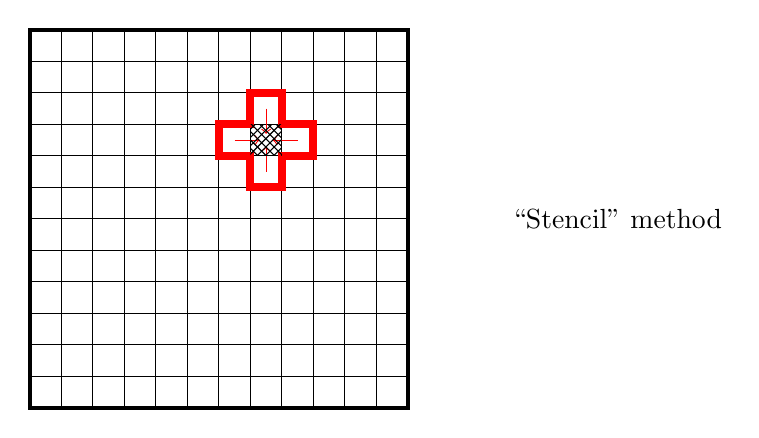
\begin{tikzpicture}[scale=0.4]
  \draw[ultra thick] (0, 0) rectangle (12, 12);
  \foreach \i in {1, 2, ..., 11} {
    \draw (\i, 0) -- +(0, 12);
    \draw (0, \i) -- +(12, 0);
  }

  \only<2>{
  \begin{scope}[xshift=2cm, yshift=2cm]
    % "croix" qui dépasse
    \draw[red, line width=1mm] (5, 5) -- ++(0, 1) -- ++ (-1, 0) -- ++(0, 1) --
    ++(1, 0) -- ++(0, 1) -- ++(1, 0) -- ++(0, -1) -- ++(1, 0) -- ++(0, -1) --
    ++(-1, 0) -- ++(0, -1) -- cycle;
    % petites flèches
    \draw[red,->] (5.5, 5.5) -- +(0, 0.8);
    \draw[red,->] (5.5, 7.5) -- +(0, -0.8);
    \draw[red,->] (4.5, 6.5) -- +(0.8, 0);
    \draw[red,->] (6.5, 6.5) -- +(-0.8, 0);
    \end{scope}
  }
    \fill<3>[pattern=crosshatch] (7, 8) rectangle +(1, 1);

    \node[anchor=west] at (15, 6) {``Stencil'' method};
  \end{tikzpicture}


\end{frame}

%%%%%%%%%%%%%%%%%%%%%%%%%%%%%%%%%%%%%%%%%%%%%%%%%%%%%%%%%%%%%%%%%%%%%%

\begin{frame}
\frametitle{``Domain Decomposition'' (a.k.a. Data Parallelism)}


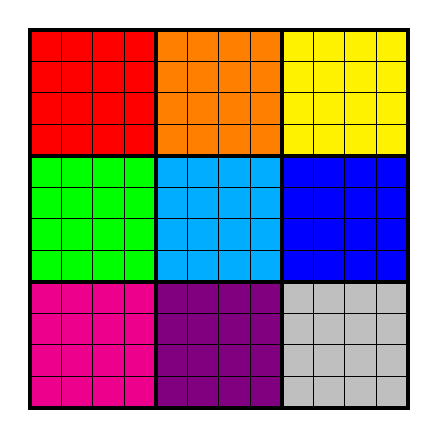
\begin{tikzpicture}[scale=0.4]
  \filldraw[very thick, fill=red]       (0, 8) rectangle  +(4, 4);
  \filldraw[very thick, fill=orange]    (4, 8) rectangle  +(4,4);
  \filldraw[very thick, fill=yellow]    (8, 8) rectangle  +(4,4);
  \filldraw[very thick, fill=green]     (0, 4) rectangle  +(4,4);
  \filldraw[very thick, fill=cyan]      (4, 4) rectangle  +(4,4);
  \filldraw[very thick, fill=blue]      (8, 4) rectangle  +(4,4);
  \filldraw[very thick, fill=magenta]   (0, 0) rectangle  +(4,4);
  \filldraw[very thick, fill=violet]    (4, 0) rectangle  +(4,4);
  \filldraw[very thick, fill=lightgray] (8, 0) rectangle  +(4,4);

  
  \draw[ultra thick] (0, 0) rectangle (12, 12);
  \foreach \i in {1, 2, ..., 11} {
    \draw (\i, 0) -- +(0, 12);
    \draw (0, \i) -- +(12, 0);
  }

  
  \end{tikzpicture}
\end{frame}

%%%%%%%%%%%%%%%%%%%%%%%%%%%%%%%%%%%%%%%%%%%%%%%%%%%%%%%%%%%%%%%%%%%%%%%%%%


\begin{frame}
\frametitle{``Domain Decomposition'' (a.k.a. Data Parallelism)}


\begin{tikzpicture}[scale=0.4]
  \path[use as bounding box] (1, 0) rectangle (18, 18);
  
  % gros carrés
  \filldraw[very thick, fill=red]       (0,  14) rectangle  +(4, 4);
  \filldraw[very thick, fill=orange]    (7,  14) rectangle  +(4,4);
  \filldraw[very thick, fill=yellow]    (14, 14) rectangle  +(4,4);
  \filldraw[very thick, fill=green]     (0,  7) rectangle  +(4,4);
  \filldraw[very thick, fill=cyan]      (7,  7) rectangle  +(4,4);
  \filldraw[very thick, fill=blue]      (14, 7) rectangle  +(4,4);
  \filldraw[very thick, fill=magenta]   (0,  0) rectangle  +(4,4);
  \filldraw[very thick, fill=violet]    (7,  0) rectangle  +(4,4);
  \filldraw[very thick, fill=lightgray] (14, 0) rectangle  +(4,4);
  
  % petites cases
  \foreach \i in {0, 1, 2} {
    \foreach \j in {0, 1, 2} {
      \foreach \k in {1, 2, 3} {
        \draw (7*\i + \k, 7*\j) -- +(0, 4);
        \draw (7*\i, 7*\j + \k) -- +(4, 0);
      }
    }
  }

  \fill<4->[pattern=crosshatch] (9, 8) rectangle +(1, 1);
  \fill<3->[pattern=crosshatch] (8, 8) rectangle +(1, 1);
  
  \begin{onlyenv}<4>
      \begin{scope}[xshift=5cm, yshift=2cm]
      % "croix" qui dépasse
      \draw[red, line width=1mm] (5, 5) -- ++(0, 1) -- ++ (-1, 0) -- ++(0, 1) --
      ++(1, 0) -- ++(0, 1) -- ++(1, 0) -- ++(0, -1) -- ++(1, 0) -- ++(0, -1) --
      ++(-1, 0) -- ++(0, -1) -- cycle;
      % petites flèches
      \draw[red,->] (5.5, 5.5) -- +(0, 0.8);
      \draw[red,->] (5.5, 7.5) -- +(0, -0.8);
      \draw[red,->] (4.5, 6.5) -- +(0.8, 0);
      \draw[red,->] (6.5, 6.5) -- +(-0.8, 0);
    \end{scope}
  \end{onlyenv}
  
  \begin{onlyenv}<3>
    \begin{scope}[xshift=4cm, yshift=2cm]
      % "croix"
      \draw[red, line width=1mm] (5, 5) -- ++(0, 1) -- ++ (-1, 0) -- ++(0, 1) --
      ++(1, 0) -- ++(0, 1) -- ++(1, 0) -- ++(0, -1) -- ++(1, 0) -- ++(0, -1) --
      ++(-1, 0) -- ++(0, -1) -- cycle;
      % petites flèches
      \draw[red,->] (5.5, 5.5) -- +(0, 0.8);
      \draw[red,->] (5.5, 7.5) -- +(0, -0.8);
      \draw[red,->] (4.5, 6.5) -- +(0.8, 0);
      \draw[red,->] (6.5, 6.5) -- +(-0.8, 0);
    \end{scope}
  \end{onlyenv}
  
  \begin{onlyenv}<2>
    \begin{scope}[xshift=3cm, yshift=2cm]
      % "croix"
      \draw[red, line width=1mm] (5, 5) -- ++(0, 1) -- ++ (-1, 0) -- ++(0, 1) --
      ++(1, 0) -- ++(0, 1) -- ++(1, 0) -- ++(0, -1) -- ++(1, 0) -- ++(0, -1) --
      ++(-1, 0) -- ++(0, -1) -- cycle;
      % petites flèches
      \draw[red,->] (5.5, 5.5) -- +(0, 0.8);
      \draw[red,->] (5.5, 7.5) -- +(0, -0.8);
      \draw[red,->] (4.5, 6.5) -- +(0.8, 0);
      \draw[red,->] (6.5, 6.5) -- +(-0.8, 0);
    \end{scope}
  \end{onlyenv}
  
  \filldraw<5>[fill=blue] (11, 7) rectangle  +(1,4);
  \draw<5> (11, 8) --  +(1,0);
  \draw<5> (11, 9) --  +(1,0);
  \draw<5> (11, 10) --  +(1,0);
  \draw<5> (11, 8) --  +(1,0);
  \draw<5>[very thick]      (7,  7) rectangle  +(5,4);  
\end{tikzpicture}
\end{frame}


%%%%%%%%%%%%%%%%%%%%%%%%%%%%%%%%%%%%%%%%%%%%%%%%%%%%%%%%%%%%%%%%%%%%%%%%%%

\begin{frame}
\frametitle{``Domain Decomposition'' (a.k.a. Data Parallelism)}

\begin{minipage}[T]{7.2cm}
\begin{tikzpicture}[scale=0.4]
  \path[use as bounding box] (1, 0) rectangle (18, 18);
  
  % halos
  \begin{onlyenv}<3->
  \filldraw[fill=violet]    (4, 0) rectangle  +(1,4);
  \filldraw[fill=magenta]   (6, 0) rectangle  +(1,4);
  \filldraw[fill=lightgray] (11, 0) rectangle  +(1,4);
  \filldraw[fill=violet]    (13, 0) rectangle  +(1,4);
  \filldraw[fill=cyan]    (4, 7) rectangle  +(1,4);
  \filldraw[fill=green]   (6, 7) rectangle  +(1,4);
  \filldraw[fill=blue] (11, 7) rectangle  +(1,4);
  \filldraw[fill=cyan]    (13, 7) rectangle  +(1,4);
  \filldraw[fill=orange]    (4, 14) rectangle  +(1,4);
  \filldraw[fill=red]   (6, 14) rectangle  +(1,4);
  \filldraw[fill=yellow]    (11,14) rectangle  +(1,4);
  \filldraw[fill=orange]    (13,14) rectangle  +(1,4);
  
  \filldraw[fill=blue]      (14, 4) rectangle  +(4,1);
  \filldraw[fill=cyan]      (7, 4) rectangle  +(4,1);
  \filldraw[fill=green]      (0, 4) rectangle  +(4,1);
  \filldraw[fill=lightgray]   (14, 6) rectangle  +(4,1);
  \filldraw[fill=violet]      (7, 6) rectangle  +(4,1);
  \filldraw[fill=magenta]     (0, 6) rectangle  +(4,1);  
  \filldraw[fill=blue]      (14, 13) rectangle  +(4,1);
  \filldraw[fill=cyan]      (7, 13) rectangle  +(4,1);
  \filldraw[fill=green]      (0, 13) rectangle  +(4,1);
  \filldraw[fill=yellow]      (14, 11) rectangle  +(4,1);
  \filldraw[fill=orange]      (7, 11) rectangle  +(4,1);
  \filldraw[fill=red]      (0, 11) rectangle  +(4,1);
\end{onlyenv}

  % gros carrés
    \filldraw[very thick, fill=red]       (0,  14) rectangle  +(4, 4);
    \filldraw[very thick, fill=orange]    (7,  14) rectangle  +(4,4);
    \filldraw[very thick, fill=yellow]    (14, 14) rectangle  +(4,4);
    \filldraw[very thick, fill=green]     (0,  7) rectangle  +(4,4);
    \filldraw[very thick, fill=cyan]      (7,  7) rectangle  +(4,4);
    \filldraw[very thick, fill=blue]      (14, 7) rectangle  +(4,4);
    \filldraw[very thick, fill=magenta]   (0,  0) rectangle  +(4,4);
    \filldraw[very thick, fill=violet]    (7,  0) rectangle  +(4,4);
    \filldraw[very thick, fill=lightgray] (14, 0) rectangle  +(4,4);
  
  \begin{onlyenv}<4->
    \draw[pattern=crosshatch, pattern color=black, very thick]       (0,  14) rectangle  +(4, 4);
    \draw[pattern=crosshatch, pattern color=black, very thick]    (7,  14) rectangle  +(4,4);
    \draw[pattern=crosshatch, pattern color=black, very thick]    (14, 14) rectangle  +(4,4);
    \draw[pattern=crosshatch, pattern color=black, very thick]     (0,  7) rectangle  +(4,4);
    \draw[pattern=crosshatch, pattern color=black, very thick]      (7,  7) rectangle  +(4,4);
    \draw[pattern=crosshatch, pattern color=black, very thick]      (14, 7) rectangle  +(4,4);
    \draw[pattern=crosshatch, pattern color=black, very thick]   (0,  0) rectangle  +(4,4);
    \draw[pattern=crosshatch, pattern color=black, very thick]    (7,  0) rectangle  +(4,4);
    \draw[pattern=crosshatch, pattern color=black, very thick] (14, 0) rectangle  +(4,4);
  \end{onlyenv}
  
  % hachures

  % petites cases, sans halo
  \begin{onlyenv}<1-2>
    \foreach \i in {0, 1, 2} {
      \foreach \j in {0, 1, 2} {
        \foreach \k in {1, 2, 3} {
          \draw (7*\i + \k, 7*\j) -- +(0, 4);
          \draw (7*\i, 7*\j + \k) -- +(4, 0);
        }
      }
    }
  \end{onlyenv}

  \begin{onlyenv}<3->
  % petites cases, halos compris
  \foreach \k in {1, 2, 3} {
    \draw (\k, 0) -- +(0, 5);
    \draw (0, \k) -- +(5, 0);
  }
  \foreach \k in {1, 2, 3} {
    \draw (\k, 6) -- +(0, 6);
    \draw (0, 7 + \k) -- +(5, 0);
  }
  \foreach \k in {1, 2, 3, 4} {
    \draw (\k, 13) -- +(0, 5);
    \draw (0, 13 + \k) -- +(5, 0);
  }
  \foreach \k in {1, 2, 3} {
    \draw (7 + \k, 0) -- +(0, 5);
    \draw (6, \k) -- +(6, 0);
  }
  \foreach \k in {1, 2, 3} {
    \draw (7 + \k, 6) -- +(0, 6);
    \draw (6, 7 + \k) -- +(6, 0);
  }
  \foreach \k in {1, 2, 3} {
    \draw (7 + \k, 13) -- +(0, 5);
    \draw (6, 14 + \k) -- +(6, 0);
  }
  \foreach \k in {1, 2, 3} {
    \draw (14 + \k, 0) -- +(0, 5);
    \draw (13, \k) -- +(5, 0);
  }
  \foreach \k in {1, 2, 3} {
    \draw (14 + \k, 6) -- +(0, 6);
    \draw (13, 7 + \k) -- +(5, 0);
  }
  \foreach \k in {1, 2, 3} {
    \draw (14 + \k, 13) -- +(0, 5);
    \draw (13, 14 + \k) -- +(5, 0);
  }
\end{onlyenv}

% flèches des halos
  \begin{onlyenv}<2,5>
 \begin{scope}[xshift=0cm, yshift=14cm]
   \draw[red, ultra thick, ->] (3.5, 0) to[bend right=20mm] +(2.5, 0);
   \draw[red, ultra thick, ->] (0, 0.5) to[bend right=20mm] +(0, -2.5);
 \end{scope}
 \begin{scope}[xshift=7cm, yshift=14cm]
   \draw[orange, ultra thick, ->] (3.5, 0) to[bend right=20mm] +(2.5, 0);
   \draw[orange, ultra thick, ->] (0.5, 4) to[bend right=20mm] +(-2.5, 0);
   \draw[orange, ultra thick, ->] (0, 0.5) to[bend right=20mm] +(0, -2.5);
 \end{scope}
 \begin{scope}[xshift=14cm, yshift=14cm]
   \draw[yellow, ultra thick, ->] (0.5, 4) to[bend right=20mm] +(-2.5, 0);
   \draw[yellow, ultra thick, ->] (0, 0.5) to[bend right=20mm] +(0, -2.5);
 \end{scope}

 \begin{scope}[xshift=0cm, yshift=7cm]
 \draw[green, ultra thick, ->] (3.5, 0) to[bend right=20mm] +(2.5, 0);
 \draw[green, ultra thick, ->] (0, 0.5) to[bend right=20mm] +(0, -2.5);
 \draw[green, ultra thick, ->] (4, 3.5) to[bend right=20mm] +(0, 2.5);
\end{scope}
 \begin{scope}[xshift=7cm, yshift=7cm]
 \draw[cyan, ultra thick, ->] (3.5, 0) to[bend right=20mm] +(2.5, 0);
 \draw[cyan, ultra thick, ->] (0.5, 4) to[bend right=20mm] +(-2.5, 0);
 \draw[cyan, ultra thick, ->] (0, 0.5) to[bend right=20mm] +(0, -2.5);
 \draw[cyan, ultra thick, ->] (4, 3.5) to[bend right=20mm] +(0, 2.5);
\end{scope}
  \begin{scope}[xshift=14cm, yshift=7cm]
 \draw[blue, ultra thick, ->] (0.5, 4) to[bend right=20mm] +(-2.5, 0);
 \draw[blue, ultra thick, ->] (0, 0.5) to[bend right=20mm] +(0, -2.5);
 \draw[blue, ultra thick, ->] (4, 3.5) to[bend right=20mm] +(0, 2.5);
\end{scope}
 \begin{scope}[xshift=0cm, yshift=0cm]
 \draw[magenta, ultra thick, ->] (3.5, 0) to[bend right=20mm] +(2.5, 0);
 \draw[magenta, ultra thick, ->] (4, 3.5) to[bend right=20mm] +(0, 2.5);
\end{scope}
 \begin{scope}[xshift=7cm, yshift=0cm]
 \draw[violet, ultra thick, ->] (3.5, 0) to[bend right=20mm] +(2.5, 0);
 \draw[violet, ultra thick, ->] (0.5, 4) to[bend right=20mm] +(-2.5, 0);
 \draw[violet, ultra thick, ->] (4, 3.5) to[bend right=20mm] +(0, 2.5);
\end{scope}
  \begin{scope}[xshift=14cm, yshift=0cm]
 \draw[lightgray, ultra thick, ->] (0.5, 4) to[bend right=20mm] +(-2.5, 0);
 \draw[lightgray, ultra thick, ->] (4, 3.5) to[bend right=20mm] +(0, 2.5);
\end{scope}
\end{onlyenv}

\end{tikzpicture}%
\end{minipage}\begin{minipage}[T]{4.5cm}
  Each processor:
  \medskip
  \begin{itemize}
  \item<1-> Knows $T$ at time~$t$
  \item<2-> Sends/Receives the \alert{halo} from its neighbors
  \item<4-> Compute $T$ at time $t + \Delta t$
  \item<5-> Rinse, repeat
  \end{itemize}

  \medskip

  \begin{alertblock}<6>{Problem}
    Progress blocked by communications
  \end{alertblock}
\end{minipage}
\end{frame}


%%%%%%%%%%%%%%%%%%%%%%%%%%%%%%%%%%%%%%%%

\begin{frame}
\frametitle{``Domain Decomposition'' (a.k.a. Data Parallelism)}

\begin{minipage}[T]{7.2cm}
\begin{tikzpicture}[scale=0.4]
  \path[use as bounding box] (1, 0) rectangle (18, 18);
  
  % halos
  \begin{onlyenv}<4->
  \filldraw[fill=violet]    (4, 0) rectangle  +(1,4);
  \filldraw[fill=magenta]   (6, 0) rectangle  +(1,4);
  \filldraw[fill=lightgray] (11, 0) rectangle  +(1,4);
  \filldraw[fill=violet]    (13, 0) rectangle  +(1,4);
  \filldraw[fill=cyan]    (4, 7) rectangle  +(1,4);
  \filldraw[fill=green]   (6, 7) rectangle  +(1,4);
  \filldraw[fill=blue] (11, 7) rectangle  +(1,4);
  \filldraw[fill=cyan]    (13, 7) rectangle  +(1,4);
  \filldraw[fill=orange]    (4, 14) rectangle  +(1,4);
  \filldraw[fill=red]   (6, 14) rectangle  +(1,4);
  \filldraw[fill=yellow]    (11,14) rectangle  +(1,4);
  \filldraw[fill=orange]    (13,14) rectangle  +(1,4);
  
  \filldraw[fill=blue]      (14, 4) rectangle  +(4,1);
  \filldraw[fill=cyan]      (7, 4) rectangle  +(4,1);
  \filldraw[fill=green]      (0, 4) rectangle  +(4,1);
  \filldraw[fill=lightgray]   (14, 6) rectangle  +(4,1);
  \filldraw[fill=violet]      (7, 6) rectangle  +(4,1);
  \filldraw[fill=magenta]     (0, 6) rectangle  +(4,1);  
  \filldraw[fill=blue]      (14, 13) rectangle  +(4,1);
  \filldraw[fill=cyan]      (7, 13) rectangle  +(4,1);
  \filldraw[fill=green]      (0, 13) rectangle  +(4,1);
  \filldraw[fill=yellow]      (14, 11) rectangle  +(4,1);
  \filldraw[fill=orange]      (7, 11) rectangle  +(4,1);
  \filldraw[fill=red]      (0, 11) rectangle  +(4,1);
\end{onlyenv}

  % gros carrés
    \filldraw[very thick, fill=red]       (0,  14) rectangle  +(4, 4);
    \filldraw[very thick, fill=orange]    (7,  14) rectangle  +(4,4);
    \filldraw[very thick, fill=yellow]    (14, 14) rectangle  +(4,4);
    \filldraw[very thick, fill=green]     (0,  7) rectangle  +(4,4);
    \filldraw[very thick, fill=cyan]      (7,  7) rectangle  +(4,4);
    \filldraw[very thick, fill=blue]      (14, 7) rectangle  +(4,4);
    \filldraw[very thick, fill=magenta]   (0,  0) rectangle  +(4,4);
    \filldraw[very thick, fill=violet]    (7,  0) rectangle  +(4,4);
    \filldraw[very thick, fill=lightgray] (14, 0) rectangle  +(4,4);
  
  \begin{onlyenv}<3-4>
    \draw[pattern=crosshatch, pattern color=black, very thick]    (1,  15) rectangle  +(2, 2);
    \draw[pattern=crosshatch, pattern color=black, very thick]    (8,  15) rectangle +(2, 2);
    \draw[pattern=crosshatch, pattern color=black, very thick]    (15, 15) rectangle +(2, 2);
    \draw[pattern=crosshatch, pattern color=black, very thick]    (1,  8) rectangle  +(2, 2);
    \draw[pattern=crosshatch, pattern color=black, very thick]    (8,  8) rectangle  +(2, 2);
    \draw[pattern=crosshatch, pattern color=black, very thick]    (15, 8) rectangle  +(2, 2);
    \draw[pattern=crosshatch, pattern color=black, very thick]    (1,  1) rectangle  +(2, 2);
    \draw[pattern=crosshatch, pattern color=black, very thick]    (8,  1) rectangle  +(2, 2);
    \draw[pattern=crosshatch, pattern color=black, very thick]    (15, 1) rectangle  +(2, 2);
  \end{onlyenv}

    \begin{onlyenv}<5->
    \draw[pattern=crosshatch, pattern color=black, very thick]       (0,  14) rectangle  +(4, 4);
    \draw[pattern=crosshatch, pattern color=black, very thick]    (7,  14) rectangle  +(4,4);
    \draw[pattern=crosshatch, pattern color=black, very thick]    (14, 14) rectangle  +(4,4);
    \draw[pattern=crosshatch, pattern color=black, very thick]     (0,  7) rectangle  +(4,4);
    \draw[pattern=crosshatch, pattern color=black, very thick]      (7,  7) rectangle  +(4,4);
    \draw[pattern=crosshatch, pattern color=black, very thick]      (14, 7) rectangle  +(4,4);
    \draw[pattern=crosshatch, pattern color=black, very thick]   (0,  0) rectangle  +(4,4);
    \draw[pattern=crosshatch, pattern color=black, very thick]    (7,  0) rectangle  +(4,4);
    \draw[pattern=crosshatch, pattern color=black, very thick] (14, 0) rectangle  +(4,4);
  \end{onlyenv}
  
  % hachures

  % petites cases, sans halo
  \begin{onlyenv}<1-3>
    \foreach \i in {0, 1, 2} {
      \foreach \j in {0, 1, 2} {
        \foreach \k in {1, 2, 3} {
          \draw (7*\i + \k, 7*\j) -- +(0, 4);
          \draw (7*\i, 7*\j + \k) -- +(4, 0);
        }
      }
    }
  \end{onlyenv}

  \begin{onlyenv}<4->
  % petites cases, halos compris
  \foreach \k in {1, 2, 3} {
    \draw (\k, 0) -- +(0, 5);
    \draw (0, \k) -- +(5, 0);
  }
  \foreach \k in {1, 2, 3} {
    \draw (\k, 6) -- +(0, 6);
    \draw (0, 7 + \k) -- +(5, 0);
  }
  \foreach \k in {1, 2, 3, 4} {
    \draw (\k, 13) -- +(0, 5);
    \draw (0, 13 + \k) -- +(5, 0);
  }
  \foreach \k in {1, 2, 3} {
    \draw (7 + \k, 0) -- +(0, 5);
    \draw (6, \k) -- +(6, 0);
  }
  \foreach \k in {1, 2, 3} {
    \draw (7 + \k, 6) -- +(0, 6);
    \draw (6, 7 + \k) -- +(6, 0);
  }
  \foreach \k in {1, 2, 3} {
    \draw (7 + \k, 13) -- +(0, 5);
    \draw (6, 14 + \k) -- +(6, 0);
  }
  \foreach \k in {1, 2, 3} {
    \draw (14 + \k, 0) -- +(0, 5);
    \draw (13, \k) -- +(5, 0);
  }
  \foreach \k in {1, 2, 3} {
    \draw (14 + \k, 6) -- +(0, 6);
    \draw (13, 7 + \k) -- +(5, 0);
  }
  \foreach \k in {1, 2, 3} {
    \draw (14 + \k, 13) -- +(0, 5);
    \draw (13, 14 + \k) -- +(5, 0);
  }
\end{onlyenv}

% flèches des halos
  \begin{onlyenv}<2-3,6>
 \begin{scope}[xshift=0cm, yshift=14cm]
   \draw[red, ultra thick, ->] (3.5, 0) to[bend right=20mm] +(2.5, 0);
   \draw[red, ultra thick, ->] (0, 0.5) to[bend right=20mm] +(0, -2.5);
 \end{scope}
 \begin{scope}[xshift=7cm, yshift=14cm]
   \draw[orange, ultra thick, ->] (3.5, 0) to[bend right=20mm] +(2.5, 0);
   \draw[orange, ultra thick, ->] (0.5, 4) to[bend right=20mm] +(-2.5, 0);
   \draw[orange, ultra thick, ->] (0, 0.5) to[bend right=20mm] +(0, -2.5);
 \end{scope}
 \begin{scope}[xshift=14cm, yshift=14cm]
   \draw[yellow, ultra thick, ->] (0.5, 4) to[bend right=20mm] +(-2.5, 0);
   \draw[yellow, ultra thick, ->] (0, 0.5) to[bend right=20mm] +(0, -2.5);
 \end{scope}

 \begin{scope}[xshift=0cm, yshift=7cm]
 \draw[green, ultra thick, ->] (3.5, 0) to[bend right=20mm] +(2.5, 0);
 \draw[green, ultra thick, ->] (0, 0.5) to[bend right=20mm] +(0, -2.5);
 \draw[green, ultra thick, ->] (4, 3.5) to[bend right=20mm] +(0, 2.5);
\end{scope}
 \begin{scope}[xshift=7cm, yshift=7cm]
 \draw[cyan, ultra thick, ->] (3.5, 0) to[bend right=20mm] +(2.5, 0);
 \draw[cyan, ultra thick, ->] (0.5, 4) to[bend right=20mm] +(-2.5, 0);
 \draw[cyan, ultra thick, ->] (0, 0.5) to[bend right=20mm] +(0, -2.5);
 \draw[cyan, ultra thick, ->] (4, 3.5) to[bend right=20mm] +(0, 2.5);
\end{scope}
  \begin{scope}[xshift=14cm, yshift=7cm]
 \draw[blue, ultra thick, ->] (0.5, 4) to[bend right=20mm] +(-2.5, 0);
 \draw[blue, ultra thick, ->] (0, 0.5) to[bend right=20mm] +(0, -2.5);
 \draw[blue, ultra thick, ->] (4, 3.5) to[bend right=20mm] +(0, 2.5);
\end{scope}
 \begin{scope}[xshift=0cm, yshift=0cm]
 \draw[magenta, ultra thick, ->] (3.5, 0) to[bend right=20mm] +(2.5, 0);
 \draw[magenta, ultra thick, ->] (4, 3.5) to[bend right=20mm] +(0, 2.5);
\end{scope}
 \begin{scope}[xshift=7cm, yshift=0cm]
 \draw[violet, ultra thick, ->] (3.5, 0) to[bend right=20mm] +(2.5, 0);
 \draw[violet, ultra thick, ->] (0.5, 4) to[bend right=20mm] +(-2.5, 0);
 \draw[violet, ultra thick, ->] (4, 3.5) to[bend right=20mm] +(0, 2.5);
\end{scope}
  \begin{scope}[xshift=14cm, yshift=0cm]
 \draw[lightgray, ultra thick, ->] (0.5, 4) to[bend right=20mm] +(-2.5, 0);
 \draw[lightgray, ultra thick, ->] (4, 3.5) to[bend right=20mm] +(0, 2.5);
\end{scope}
\end{onlyenv}

\end{tikzpicture}%
\end{minipage}\begin{minipage}[T]{4.5cm}
  Each processor:
  \medskip
  \begin{itemize}
  \item<1-> Knows $T$ at time~$t$
  \item<2-> Sends the \alert{halo} to its neighbors (\alert{Isend})
  \item<3-> Compute $T$ at time $t + \Delta t$ (\alert{interior})
  \item<4-> Waits end of comms
  \item<5-> Compute $T$ at time $t + \Delta t$ (\alert{border})
  \item<6-> Rinse, repeat
  \end{itemize}
\end{minipage}
\end{frame}

%%%%%%%%%%%%%%%%%%%%%%%

\begin{frame}[fragile=singleslide]

\begin{wider}
\begin{minted}[fontsize=\footnotesize]{C}
int MPI_Sendrecv(void *sendbuf, int sendcount, MPI_Datatype sendtype, 
                 int dest, int sendtag, 
                 void *recvbuf, int recvcount, MPI_Datatype recvtype, 
                 int source, int recvtag, 
                 MPI_Comm comm, MPI_Status *status);
\end{minted}
\end{wider}

\begin{wider}
\begin{minted}[fontsize=\footnotesize]{C}
int MPI_Isend(void *buf, int count, MPI_Datatype datatype, 
              int dest, int tag, 
              MPI_Comm comm, MPI_Request *request);
int MPI_Irecv(void *buf, int count, MPI_Datatype datatype,
              int source, int tag, 
              MPI_Comm comm, MPI_Request *request);
int MPI_Waitall(int count, 
                MPI_Request requests[], MPI_Status statuses[]);
\end{minted}
\end{wider}

\begin{alertblock}{warning!}
  \begin{itemize}    
  \item East / West border: \alert{non-contiguous} data elements
    \item[$\Rightarrow$] Must create \alert{derived MPI types} (\mintinline{C}{MPI_Type_vector(...)})
  \end{itemize}
\end{alertblock}
\end{frame}


%%%%%%%%%%%%%%%%%%%%%%%%%%%%%%%%%%%%%%%%%%%%%%%%%%%%%%%%%%%%%%%%%%%%%%%%%%

\section{Prefix-Sum}

\begin{frame}[fragile]
\frametitle{Parallélisme de données}


\begin{block}{Exemple classique : \emph{prefix-sum} (``scan'') (en place)}
\begin{minted}{C}
for (int i = 1; i < n; i++)
    A[i] = A[i] + A[i - 1];
\end{minted}
\end{block}

\bigskip

\begin{itemize}
\item \textbf{Dépendance de données}
\item Chaque itération a besoin du résultat de la précédente...
\item Changer l'algorithme   
\end{itemize}
\end{frame}

%%%%%%%%%%%%%%%%%%%%%%%%%%%%%%%%%%%%%%%%%%%%%%%%%%%%%%%%%%%%%%%%

\begin{frame}[fragile]
\frametitle{\texttt{prefix-sum} : Cas de la mémoire partagée}


\begin{block}{Exemple classique : \emph{prefix-sum} (en place)}
\begin{minted}[fontsize=\small]{C}
double *B;

void prefix_sum(double * A, int n)
{
    if (n < 2)
        return;
    for (int i = 0; i < n / 2; i++)
        B[i] = A[2 * i] + A[2 * i + 1];
    prefix_sum(B, k);
    for (int i = 1; i < n; i += 2) {
          A[i] = B[i / 2];
          A[i + 1] = B[i / 2] + A[i + 1];
    }
}
\end{minted}
\end{block}


\end{frame}


%%%%%%%%%%%%%%%%%%%%%%%%%%%%%%%%%%%%%%%%%%%%%%%%%%%%%%%%%%%%%%%%%

\begin{frame}
\frametitle{Algorithme MIMD-DM pour \texttt{prefix-sum}}

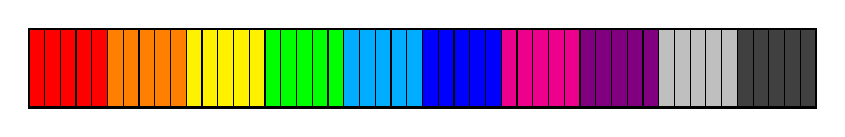
\begin{tikzpicture}
  \filldraw[fill=red]    (0, 0) rectangle  +(1,1);
  \filldraw[fill=orange] (1, 0) rectangle  +(1,1);
  \filldraw[fill=yellow] (2, 0) rectangle  +(1,1);
  \filldraw[fill=green]  (3, 0) rectangle  +(1,1);
  \filldraw[fill=cyan]   (4, 0) rectangle  +(1,1);
  \filldraw[fill=blue]   (5, 0) rectangle  +(1,1);
  \filldraw[fill=magenta] (6, 0) rectangle  +(1,1);
  \filldraw[fill=violet] (7, 0) rectangle +(1,1);
  \filldraw[fill=lightgray] (8, 0) rectangle +(1,1);
  \filldraw[fill=darkgray] (9, 0) rectangle +(1,1);
  
  \draw[thick] (0, 0) rectangle (10, 1);
  \foreach \i in {0.2, 0.4, ..., 9.8}
  \draw (\i, 0) -- +(0, 1);
\end{tikzpicture}

\bigskip

\begin{enumerate}
\item $P_i$ calcule la somme $S_i$ de \emph{ses} données. \hfill \alert{[local]}
\item Ils font (collectivement) $T \gets \texttt{prefix-sum}(S)$.
  \begin{itemize}
  \item \texttt{MPI\_Scan}
  \end{itemize}
\item[$\rightarrow$] $P_i$ obtient $T_i = $ somme des données des $P_j$ (pour $j<i$).
\item $P_i$ \texttt{prefix-sum} ses données en ajoutant $T_i$. \hfill \alert{[local]}
\end{enumerate}
\end{frame}

%%%%%%%%%%%%%%%%%%%%%%%%%%%%%%%%%%%%%%%%% 

\begin{frame}
  \frametitle{Rappel : \texttt{reduce} par la méthode de l'arbre binomial}
  
  \begin{center}
    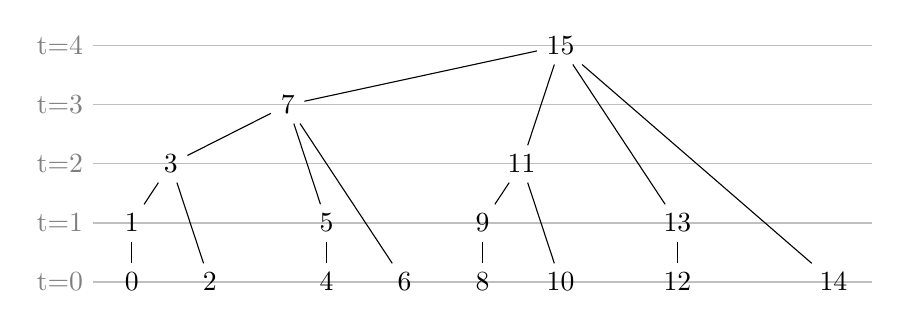
\begin{tikzpicture}[level distance=10mm, xscale=0.66, yscale=0.75]
  \foreach \i in {0,1,2,3,4} {
    \draw[semitransparent,gray] (-9, -4+\i) node[text=black,left] {t=\i} -- +(15, 0);
  }

  \node {15}
    child { node {7}
      child { node {3}
        child {node {1}
          child {node {0}}
        }
        child {node at (0, -1) {2}}
      }
      child[missing]
      child {node at (0,-1) {5}
        child {node {4}}
      }
      child {node at (0,-2) {6} }
    }
    child[missing]
    child[missing]
    child { node at (0, -1) {11}
      child {node {9}
        child {node {8} }
      }
      child {node at (0, -1) {10} }
    }
    child[missing]
    child { node at (0, -2) {13}
      child {node {12}}
    }
    child[missing]
    child { node at (0, -3) {14} }
;
\end{tikzpicture}
\end{center}


  \begin{center}
    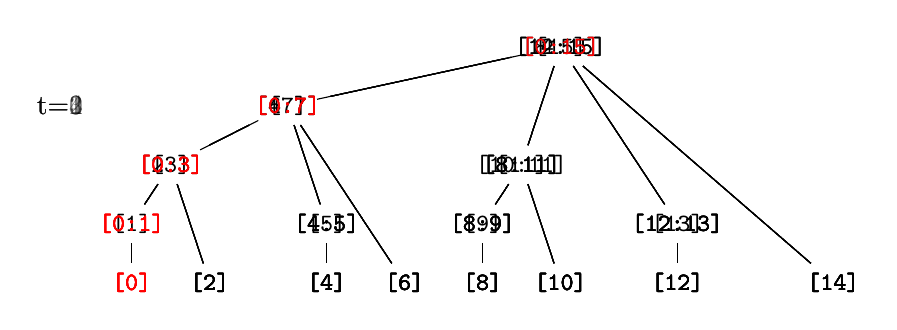
\begin{tikzpicture}[level distance=10mm, xscale=0.66, yscale=0.75]

      %%%
      \path<1> [semitransparent,gray] (-9, -1) node[text=black,left] {t=0};
      \path<2> [semitransparent,gray] (-9, -1) node[text=black,left] {t=1};
      \path<3> [semitransparent,gray] (-9, -1) node[text=black,left] {t=2};
      \path<4> [semitransparent,gray] (-9, -1) node[text=black,left] {t=3};
      \path<5> [semitransparent,gray] (-9, -1) node[text=black,left] {t=4};
      
      \begin{scope}[every node/.style={font=\small\ttfamily}]
          \node<1> {[15]}
    child { node {[7]}
      child { node {[3]}
        child {node {[1]}
          child {node[text=red] {[0]}}
        }
        child {node at (0, -1) {[2]}}
      }
      child[missing]
      child {node at (0,-1) {[5]}
        child {node {[4]}}
      }
      child {node at (0,-2) {[6]} }
    }
    child[missing]
    child[missing]
    child { node at (0, -1) {[11]}
      child {node {[9]}
        child {node {[8]} }
      }
      child {node at (0, -1) {[10]} }
    }
    child[missing]
    child { node at (0, -2) {[13]}
      child {node {[12]}}
    }
    child[missing]
    child { node at (0, -3) {[14]} }
    ;
    
    %%%%%%

    \node<2> {[14:15]}
    child { node {[6:7]}
      child { node {[2:3]}
        child {node[text=red] {[0:1]}
          child {node[text=red] {[0]}}
        }
        child {node at (0, -1) {[2]}}
      }
      child[missing]
      child {node at (0,-1) {[4:5]}
        child {node {[4]}}
      }
      child {node at (0,-2) {[6]} }
    }
    child[missing]
    child[missing]
    child { node at (0, -1) {[10:11]}
      child {node {[8:9]}
        child {node {[8]} }
      }
      child {node at (0, -1) {[10]} }
    }
    child[missing]
    child { node at (0, -2) {[12:13]}
      child {node {[12]}}
    }
    child[missing]
    child { node at (0, -3) {[14]} }
    ;

    %%%%%% 

    \node<3> {[12:15]}
    child { node {[4:7]}
      child { node [text=red] {[0:3]}
        child {node[text=red] {[0:1]}
          child {node[text=red] {[0]}}
        }
        child {node at (0, -1) {[2]}}
      }
      child[missing]
      child {node at (0,-1) {[4:5]}
        child {node {[4]}}
      }
      child {node at (0,-2) {[6]} }
    }
    child[missing]
    child[missing]
    child { node at (0, -1) {[8:11]}
      child {node {[8:9]}
        child {node {[8]} }
      }
      child {node at (0, -1) {[10]} }
    }
    child[missing]
    child { node at (0, -2) {[12:13]}
      child {node {[12]}}
    }
    child[missing]
    child { node at (0, -3) {[14]} }
    ;

    %%%%%% 

    \node<4> {[8:15]}
    child { node[text=red] {[0:7]}
      child { node [text=red] {[0:3]}
        child {node[text=red] {[0:1]}
          child {node[text=red] {[0]}}
        }
        child {node at (0, -1) {[2]}}
      }
      child[missing]
      child {node at (0,-1) {[4:5]}
        child {node {[4]}}
      }
      child {node at (0,-2) {[6]} }
    }
    child[missing]
    child[missing]
    child { node at (0, -1) {[8:11]}
      child {node {[8:9]}
        child {node {[8]} }
      }
      child {node at (0, -1) {[10]} }
    }
    child[missing]
    child { node at (0, -2) {[12:13]}
      child {node {[12]}}
    }
    child[missing]
    child { node at (0, -3) {[14]} }
    ;

    %%%%%% 

    \node<5>[text=red] {[0:15]}
    child { node[text=red] {[0:7]}
      child { node [text=red] {[0:3]}
        child {node[text=red] {[0:1]}
          child {node[text=red] {[0]}}
        }
        child {node at (0, -1) {[2]}}
      }
      child[missing]
      child {node at (0,-1) {[4:5]}
        child {node {[4]}}
      }
      child {node at (0,-2) {[6]} }
    }
    child[missing]
    child[missing]
    child { node at (0, -1) {[8:11]}
      child {node {[8:9]}
        child {node {[8]} }
      }
      child {node at (0, -1) {[10]} }
    }
    child[missing]
    child { node at (0, -2) {[12:13]}
      child {node {[12]}}
    }
    child[missing]
    child { node at (0, -3) {[14]} }
    ;

  \end{scope}
\end{tikzpicture}
\end{center}
\end{frame}

%%%%%%%%%%%%%%%%%%%%%%%%%%%%%%%%%%%%%%%%%%%

\begin{frame}
  \frametitle{\texttt{prefix-sum} en mémoire distribuée (arbre binomial)}

  \begin{exampleblock}{Phase 1 : \texttt{reduce}}
    Chaque noeud :
    \begin{enumerate}
    \item Récupère (et stocke) les valeurs de ses enfants.
    \item Calcule la somme, ajoute sa propre valeur, envoie à son père.
    \end{enumerate}
  \end{exampleblock}

  $\rightarrow \log_2$ messages successifs.
  
  \medskip

  \begin{alertblock}{Phase 2 : \texttt{prefix-sum}}
    Chaque noeud :
    \begin{enumerate}
    \item Reçoit une valeur de son père
      \begin{itemize}
      \item Somme des valeurs de ses frères \emph{gauches}.
        
      \end{itemize}
      
    \item Envoie à chacun de ses fils la somme des valeurs remontées par ses
      frères \emph{gauches}, plus la valeur reçue du père.
    \end{enumerate}
  \end{alertblock}

    $\rightarrow \log_2$ messages successifs.
\end{frame}

%%%%%%%%%%%%%%%%%%%%%%%%%%%%%%%%%%%

\begin{frame}<5->
  \frametitle{\texttt{prefix-sum} par la méthode de l'arbre binomial}
  

  \begin{center}
    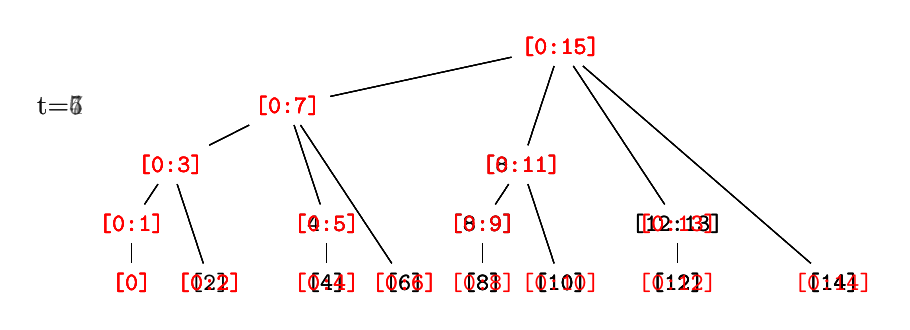
\begin{tikzpicture}[level distance=10mm, xscale=0.66, yscale=0.75]

      %%%
    \path<5> [semitransparent,gray] (-9, -1) node[text=black,left] {t=4};
    \path<6> [semitransparent,gray] (-9, -1) node[text=black,left] {t=5};
    \path<7> [semitransparent,gray] (-9, -1) node[text=black,left] {t=6};
    \path<8> [semitransparent,gray] (-9, -1) node[text=black,left] {t=7};
    
      \begin{scope}[every node/.style={font=\small\ttfamily}]

    \node<5>[text=red] {[0:15]}
    child { node[text=red] {[0:7]}
      child { node [text=red] {[0:3]}
        child {node[text=red] {[0:1]}
          child {node[text=red] {[0]}}
        }
        child {node at (0, -1) {[2]}}
      }
      child[missing]
      child {node at (0,-1) {[4:5]}
        child {node {[4]}}
      }
      child {node at (0,-2) {[6]} }
    }
    child[missing]
    child[missing]
    child { node at (0, -1) {[8:11]}
      child {node {[8:9]}
        child {node {[8]} }
      }
      child {node at (0, -1) {[10]} }
    }
    child[missing]
    child { node at (0, -2) {[12:13]}
      child {node {[12]}}
    }
    child[missing]
    child { node at (0, -3) {[14]} }
    ;


        \node<6>[text=red] {[0:15]}
    child { node[text=red] {[0:7]}
      child { node [text=red] {[0:3]}
        child {node[text=red] {[0:1]}
          child {node[text=red] {[0]}}
        }
        child {node[text=red] at (0, -1) {[0:2]}}
      }
      child[missing]
      child {node[text=red] at (0,-1) {[0:5]}
        child {node {[4]}}
      }
      child {node at (0,-2) {[6]} }
    }
    child[missing]
    child[missing]
    child { node[text=red] at (0, -1) {[0:11]}
      child {node {[8:9]}
        child {node {[8]} }
      }
      child {node at (0, -1) {[10]} }
    }
    child[missing]
    child { node at (0, -2) {[12:13]}
      child {node {[12]}}
    }
    child[missing]
    child { node at (0, -3) {[14]} }
    ;

    \node<7>[text=red] {[0:15]}
    child { node[text=red] {[0:7]}
      child { node [text=red] {[0:3]}
        child {node[text=red] {[0:1]}
          child {node[text=red] {[0]}}
        }
        child {node[text=red] at (0, -1) {[0:2]}}
      }
      child[missing]
      child {node[text=red] at (0,-1) {[0:5]}
        child {node[text=red] {[0:4]}}
      }
      child {node[text=red] at (0,-2) {[0:6]} }
    }
    child[missing]
    child[missing]
    child { node[text=red] at (0, -1) {[0:11]}
      child {node[text=red] {[0:9]}
        child {node {[8]} }
      }
      child {node at (0, -1) {[10]} }
    }
    child[missing]
    child { node[text=red] at (0, -2) {[0:13]}
      child {node {[12]}}
    }
    child[missing]
    child { node at (0, -3) {[14]} }
    ;

    \node<8>[text=red] {[0:15]}
    child { node[text=red] {[0:7]}
      child { node [text=red] {[0:3]}
        child {node[text=red] {[0:1]}
          child {node[text=red] {[0]}}
        }
        child {node[text=red] at (0, -1) {[0:2]}}
      }
      child[missing]
      child {node[text=red] at (0,-1) {[0:5]}
        child {node[text=red] {[0:4]}}
      }
      child {node[text=red] at (0,-2) {[0:6]} }
    }
    child[missing]
    child[missing]
    child { node[text=red] at (0, -1) {[0:11]}
      child {node[text=red] {[0:9]}
        child {node[text=red] {[0:8]} }
      }
      child {node[text=red] at (0, -1) {[0:10]} }
    }
    child[missing]
    child { node[text=red] at (0, -2) {[0:13]}
      child {node[text=red] {[0:12]}}
    }
    child[missing]
    child { node[text=red] at (0, -3) {[0:14]} }
    ;

  \end{scope}
\end{tikzpicture}
\end{center}
\end{frame}



\end{document}






% Charles' emacs magic commands
%%% Local Variables:
%%% TeX-engine: xetex
%%% TeX-command-extra: "-shell-escape"
%%% TeX-command-extra-options: "-shell-escape"
%%% ispell-local-dictionary: "english"
%%% eval: (flyspell-mode 1)
%%% eval: (reftex-mode 1)
%%% End:
